\section{Adding a Single Adjoint scalar} \label{sec:adj}
Consider now the case of the scalar in the adjoint representation of $\mathrm{SU}(N)$. These scalars will be $N\times N$ matrices and can be written as $\Phi=\phi^bT^b$ where the scalar field transforms as $\Phi(x)\to U(x)\Phi(x)U^\dagger(x)$ with $U(x)=e^{\alpha^a(x)T^a}\in \mathrm{SU}(N)$. The adjoint representation is a real representation, consequently rendering it neutral under Abelian groups. It has $N^2-1$ degrees of freedom. 

Including an adjoint scalar when extending the SM is particularly useful for implementing spontaneous symmetry breaking. That is, if the scalar field acquires a VEV, it can lead to spontaneous symmetry breaking, e.g.\ $\mathrm{SU}(N)\to \mathrm{SU}(N-M)\times \mathrm{SU}(M)\times \mathrm{U}(1)$ \cite{Georgi:1974yf, Li:1973mq}. 


The new representation of the scalar changes the Lagrangian to
\begin{align}
    \mathcal{L}= &-\frac{1}{4} F_{\mu\nu}^a F^{a\mu\nu}+ i \bar{\Lambda}^{ij} \slashed{D} \Lambda_{ij} 
    + i \bar{\psi}^i_\alpha \slashed{D} \psi_i^\alpha 
    + i \bar{\tilde{\psi}}_i^\beta \slashed{D} \tilde{\psi}^i_\beta\nonumber\\&+\tr((D^\mu\Phi)(D_\mu\Phi))+ (y^\beta_\alpha \tilde\psi_\beta \Phi\psi^{\alpha}+h.c.)+\lambda_1\tr(\Phi^2)^2+\lambda_2\tr(\Phi^4)
    \;.\label{eq:Ladj}
\end{align}
In comparison to the previous model in Section \ref{sec:fundscalar}, an additional quartic term can be written\footnote{For $N\in\{2,3\}$ there are completeness identities which contract the indices and make the two quartic terms proportional. This is because the determinant goes as $(\Phi^2)^N$. The result of the BY model for $N=3$ can be seen in Appendix \ref{app:BYN3}, where it is shown that the change to the Lagrangian does not effect the final conclusion, the for $N=3$ the BY model is never CAF independently of the number of chiral generations. }. The transformation rules of the model can be seen in Table \ref{tab:adj}. Note that the $\mathrm{U}_2(1)$ symmetry (depending on $p$) is explicitly broken by the Yukawa term in the Lagrangian, since the adjoint scalar is neutral under Abelian groups and thus cannot render the term invariant under $\mathrm{U}_2(1)$.  

From Eq.\ \eqref{eq:Ladj} we see that the structure of the Yukawa term is changed, compared to the previous model. It no longer includes the chiral fermionic sector, but instead couples the vector-like fermions. Similar to the model in Section \ref{sec:fundscalarNg}, the Yukawa coupling is a matrix since $\tilde\psi$ and $\psi$ transform under two different groups. The dimensions of the Yukawa matrix is $p\times (N\mp 4+p)$, assuming universality as done in Section \ref{sec:fundscalarNg}, the trace factor is given by $\min(p,(N\mp 4+p))=p$ for all relevant $N$ of the two models. With this, we find the beta functions of the model to be 
\begin{align}
    \beta_g&=-\frac{1}{3}\,\alpha_g^2\left(17N \pm 12 -4p\right)\;,\\
    \beta_{y}&=\alpha_y\left[\left(\frac 6N-6N\right) \alpha_g+ 2p \alpha_{y}+ \left(N-\frac 3N\right )\alpha_y\right]\;,\\
    \beta_{\lambda_1} &=4\frac{N^2-9}{N}\alpha_{\lambda_1}^2+12\alpha_{\lambda_1}\alpha_{\lambda_2}+4(p\alpha_{y}-3\alpha_{g})\alpha_{\lambda_1}+3N\alpha_g^2-2p\alpha_{y}^2\;,
    \\
    \beta_{{\lambda_2}}&=(7+N^2)\alpha_{\lambda_2}^2+\frac{12(3+N^2)}{N^2}\alpha_{\lambda_1}^2+\frac{4(2N^2-3)}{N}\alpha_{\lambda_1}\alpha_{\lambda_2}+4(p\alpha_{y}-3N\alpha_{g})\alpha_{\lambda_2}+18\alpha_{g}^2\;.
\end{align}
 \begin{table}[ht]
    \centering
    \renewcommand{\arraystretch}{1.5} 
    \begin{tabular}{|c|c|c|c|c|}
    \hline
    Fields & $\mathrm{SU}(N)$ & $\mathrm{SU}(N \mp 4 + p)$ & $\mathrm{SU}(p)$ & $\mathrm{U}_1(1)$  \\
    \hline
    $\Lambda$ & $\ytableausetup{boxsize=0.25cm, centertableaux}\begin{ytableau}{}\\{}\end{ytableau} \;\, / \;\, \begin{ytableau}{}&{}\end{ytableau}$ & 1 & 1 & $N \mp 4$  \\

    $\tilde\psi$ & $\overline{\begin{ytableau}{}\end{ytableau}\rule{0pt}{7.5pt}}$ & $\overline{\begin{ytableau}{}\end{ytableau}\rule{0pt}{7.5pt}}$ & 1 & $-(N \mp 2)$ \\

    $\psi$ & ${\begin{ytableau}{}\end{ytableau}}$ & 1 & ${\begin{ytableau}{}\end{ytableau}}$ & $N \mp 2$  \\
    \hline
     $\phi$ & \textbf{adj} & $1$ & $1$ & $0$  \\
    \hline
    \end{tabular}
    \caption{Field content of the GG (upper signs, antisymmetric $\Lambda$) and BY (lower signs, symmetric $\Lambda$) models with an adjoint scalar $\phi$.  The table shows how the fields transform under the gauge and global symmetry groups, and their charges under the $\mathrm{U}_1(1)$ symmetry. Note that the $\mathrm{U}_2(1)$ is explicitly broken by the Yukawa term in the Lagrangian and is therefore not added to the table. }
    \label{tab:adj} 
\end{table}

In this section we will focus on the analysis for the GG model. A similar analysis applies to the BY model with results shown in Figures  \ref{fig:gg_combined_ng1} and \ref{fig:DeltaadjGG}.

Having two quartic couplings makes the CAF analysis different from the previous models and requires root analysis of fourth degree polynomials. We use the approach described in Section \ref{sec:CAF2} and Appendix \ref{sec:appCafadj}. This framework converts the task of solving coupled differential equations to an exercise of finding real positive solutions to a fourth-degree polynomial. There are three possible scenarios of real or complex roots, depending on the parameters $N$ and $p$. In Figure \ref{fig:roots_fixed}, it is evident that only complex roots are possible when the gauge coupling is asymptotically free, i.e.\ under the dashed line. In conclusion, there are no CAF solutions for the theory. 

In the regime where the Yukawa coupling vanishes faster than $1/t$, its contribution to the scalar beta functions is subleading. The UV behaviour of the theory may then be analysed by solving the gauge–scalar subsystem on fixed flow, effectively reducing the quartic beta equations to
\begin{align}
    \beta_{{\lambda_1}} &=4\frac{N^2-9}{N}\alpha_{\lambda_1}^2+12\alpha_{\lambda_1}\alpha_{\lambda_2}-12N\alpha_{g}\alpha_{\lambda_1}+3N\alpha_g^2 \;,\label{eq:beta1yoff}
    \\
    \beta_{{\lambda_2}}&=(7+N^2)\alpha_{\lambda_2}^2+\frac{12(3+N^2)}{N^2}\alpha_{\lambda_1}^2+\frac{4(2N^2-3)}{N}\alpha_{\lambda_1}\alpha_{\lambda_2}-12N\alpha_{g}\alpha_{\lambda_2}+18\alpha_{g}^2\;.\label{eq:beta12yoff}
\end{align}
This approach was explained in Section \ref{sec:CAF2}. 

\begin{figure}[ht]
    \centering
    \begin{subfigure}[b]{0.49\textwidth}
        \centering
        
\includegraphics[width=\textwidth]{Figures/CAFplotGG_1_RootsFixed_Ng1.pdf}
        \caption{All couplings on fixed flow} 
        \label{fig:roots_fixed}
    \end{subfigure}
    \hspace{0.1cm}
    \begin{subfigure}[b]{0.49\textwidth}
        \centering
        
\includegraphics[width=\textwidth]{Figures/CAFplotGG_2_RootsNoY_Ng1.pdf}
        \caption{$\alpha_y$ off fixed flow} 
        \label{fig:roots_noy}
    \end{subfigure}
    
    \caption{ Root structure of the fourth-degree polynomial for the GG model, for (a) all couplings on fixed flow and (b) the Yukawa coupling off fixed flow. The shaded regions denote four complex roots (white), and two real and two complex roots (light green). The dashed black line illustrates the $b_0=0$ condition, underneath which the gauge coupling is asymptotic free.} 
    \label{fig:Deltaadj}
\end{figure}
We can now perform a CAF analysis of these beta functions, leading to conditions for the quartic couplings and well-defined CAF regions. This can be seen in Figure \ref{fig:roots_noy}. In this case, there is a region where both the gauge coupling is asymptotically free and there are two real and two complex roots. To have a CAF region, we also require a potential bounded from below. Thus, the quartic couplings must be positive as well as real. To determine this, we can use Descartes' rule of signs. For the region shaded in Figure \ref{fig:BYposroots} there are three sign changes resulting in one positive real root, ensuring that the theory has a CAF region.

\begin{figure}[t!]
    \centering
    
\includegraphics[width=0.5\textwidth]{Figures/CAFplotGG_3_FinalCombined_Ng1.pdf}
    \caption{CAF regions for the GG model with the Yukawa coupling $\alpha_y$ off fixed flow (light blue). The dashed black line illustrates the $b_0=0$ condition (Eq.\ \eqref{eq:pmaxadj}), and the solid black line the $\Delta=0$ for $\alpha_y$ off fixed flow \eqref{eq:Delta0noY}.}
    \label{fig:BYposroots}
\end{figure}
In Figure \ref{fig:BYposroots}, the shaded region illustrates the models CAF region with the Yukawa coupling off fixed flow. A similar result can be seen for the BY model in Figure \ref{fig:gg_combined_ng1}. 

The CAF region is bounded from the top by the condition of $b_0=0$, from which we obtain the following function
\begin{align}
    p_{\max}(N)&=\frac{17N\pm12}{4}\;. \label{eq:pmaxadj}
\end{align}
The $p_{\min}$ function comes from the condition of $\Delta=0$ (see Eqs. \eqref{eq:Delta0noY} and \eqref{eq:Delta0}), where $\Delta$ is the discriminant of the fourth degree polynomial in Eq.\ \eqref{eq:fourthdegpoly}.  

As in the case of the anti-fundamental scalar, we can extend our model to include multiple chiral families. We will do this in the following section.
\subsection{Inclusion of Chiral Families}\label{sec:adjNg}
 Let us now upgrade the model with an adjoint scalar to include chiral generations. As done in Section \ref{sec:fundscalarNg}, the gauge group will depend on the number of families $\mathrm{SU}(N_g(N\mp4)+p)$. This also changes the transformation table, see Table \ref{tab:adj_Ng}. 

We obtain the Lagrangian 
\begin{align}
   \mathcal{L}= &-\frac{1}{4} F_{\mu\nu}^a F^{a\mu\nu}+ i \bar{\Lambda}^{ij\gamma} \slashed{D} \Lambda_{ij\gamma } 
    + i \bar{\psi}^i_\alpha \slashed{D} \psi_i^\alpha 
    + i \bar{\tilde{\psi}}_i^\beta \slashed{D} \tilde{\psi}^i_\beta\nonumber\\&+\tr((D^\mu\Phi)(D_\mu\Phi))+ (y^\beta_\alpha \tilde\psi_\beta \Phi\psi^{\alpha}+h.c.)+\lambda_1\tr(\Phi^2)^2+\lambda_2\tr(\Phi^4)
    \;,
\end{align}
where again the $\mathrm{U}_2(1)$ symmetry is explicitly broken.
\begin{table}[ht]
    \centering
    \renewcommand{\arraystretch}{1.5} 
    \begin{tabular}{|c|c|c|c|c|c|}
    \hline
    Fields & $\mathrm{SU}(N)$ & $\mathrm{SU}(N_g(N \mp 4) + p)$ & $\mathrm{SU}(p)$ & $\mathrm{SU}(N_g)$ & $\mathrm{U}_1(1)$  \\
    \hline
    $\Lambda$ & $\ytableausetup{boxsize=0.25cm, centertableaux}\begin{ytableau}{}\\{}\end{ytableau} \;\, / \;\, \begin{ytableau}{}&{}\end{ytableau}$ & $1$ & $1$ &$\overline{\begin{ytableau}{}\end{ytableau}\rule{0pt}{7.5pt}}$ & $N \mp 4$ \\

    $\tilde\psi$ & $\overline{\begin{ytableau}{}\end{ytableau}\rule{0pt}{7.5pt}}$ & $\overline{\begin{ytableau}{}\end{ytableau}\rule{0pt}{7.5pt}}$ & 1&1 & $-(N \mp 2)$  \\

    $\psi$ & ${\begin{ytableau}{}\end{ytableau}}$ & 1 & ${\begin{ytableau}{}\end{ytableau}}$ & 1&$N \mp 2$ \\
    \hline
    $\phi$ & \textbf{adj} & $1$ & $1$ & $1$ & $0$  \\
    \hline
    \end{tabular}
    \caption{Field content of the GG (upper signs, antisymmetric $\Lambda$) and BY (lower signs, symmetric $\Lambda$) models with $N_g$ chiral families and adjoint scalar $\phi$.  The table shows how the fields transform under the gauge and global symmetry groups, and their charges under the $\mathrm{U}_1(1)$ symmetry. Note that the $\mathrm{U}_2(1)$ is explicitly broken by the Yukawa term in the Lagrangian and is therefore not added to the table. }
    \label{tab:adj_Ng} 
\end{table}

Since, the Yukawa interaction is does not include the chiral fermions in the case of an adjoint scalar; only the gauge beta function will change
\begin{equation}
     \beta_g=-\frac{1}{3}\left(21N \pm 12 N_g-4p-4N_gN)\right)\alpha_g^2\;.\\
\end{equation} 
\begin{figure}[t!]
    \centering
    \begin{subfigure}[b]{0.49\textwidth}
        \centering
        
\includegraphics[width=\textwidth]{Figures/CAFplotGG_1_RootsFixed_Ng3.pdf}
        \caption{Real roots on fixed flow} 
        \label{fig:roots_fixed_ng2}
    \end{subfigure}
    \hspace{0.1cm}
    \begin{subfigure}[b]{0.49\textwidth}
        \centering
        
\includegraphics[width=\textwidth]{Figures/CAFplotGG_3_FinalCombined_Ng3.pdf}
        \caption{CAF region} 
        \label{fig:final_combined_ng2}
    \end{subfigure}
    
    \caption{ Properties of the GG model with $N_g=3$ chiral families. (a) Root structure of the fourth-degree polynomial with all the couplings on fixed flow. The shaded regions denote four complex roots (white) or two real and two complex roots (light green). (b) CAF regions with the Yukawa coupling $\alpha_y$ off fixed flow (light blue). The dashed black line illustrates the $b_0=0$ condition (Eq.\ \eqref{eq:pmaxadj}), and the solid black line the $\Delta=0$ for $\alpha_y$ off fixed flow \eqref{eq:Delta0noY}.} 
    \label{fig:Ng2}
\end{figure}

It is only possible to express the upper boundary in a compact analytic form, analogous to the case of a single chiral family. In this analysis, we obtain
\begin{align}
    p_{\max}(N,N_g)=\frac{21N\pm12 N_g-4NN_g}{4}\label{eq:padjscalar}
\end{align}
where the lower boundary is described by $\Delta=0$ (see Eqs. \eqref{eq:Delta0noY} and \eqref{eq:Delta0}).

Now we can perform a CAF analysis. First, consider the case of $N_g=3$. In Figure \ref{fig:Ng2}, a similar result can be seen as that for one chiral family: we need to go off fixed flow to obtain a CAF region. Figure \ref{fig:roots_fixed_ng2} illustrates that on fixed-flow, the roots will all be complex, when considering solutions below the dashed line, i.e.\ for asymptotic free gauge coupling. In Figure \ref{fig:final_combined_ng2}, the light blue region represents the CAF region for the Yukawa coupling off fixed flow. 

\begin{figure}[t!]
    \centering
    \begin{subfigure}[b]{0.49\textwidth}
        \centering
        
\includegraphics[width=\textwidth]{Figures/CAFplotGG_1_RootsFixed_Ng5.pdf}
        \caption{Real roots on fixed flow with $N_g=5$} 
        \label{fig:roots_fixed_ng3}
    \end{subfigure}
    \hspace{0.1cm}
    \begin{subfigure}[b]{0.49\textwidth}
        \centering
        
\includegraphics[width=\textwidth]{Figures/CAFplotGG_3_FinalCombined_Ng5.pdf}
        \caption{CAF region with $N_g=5$} 
        \label{fig:final_combined_ng3}
    \end{subfigure}

     \vspace{0.5cm} 
    \begin{subfigure}[b]{0.49\textwidth}
        \centering
        
\includegraphics[width=\textwidth]{Figures/CAFplotGG_3_FinalCombined_Ng6.pdf}
        \caption{CAF region with $N_g=6$} 
        \label{fig:gg_combined_ng5}
    \end{subfigure}
    \hspace{0.1cm}
    \begin{subfigure}[b]{0.49\textwidth}
        \centering
        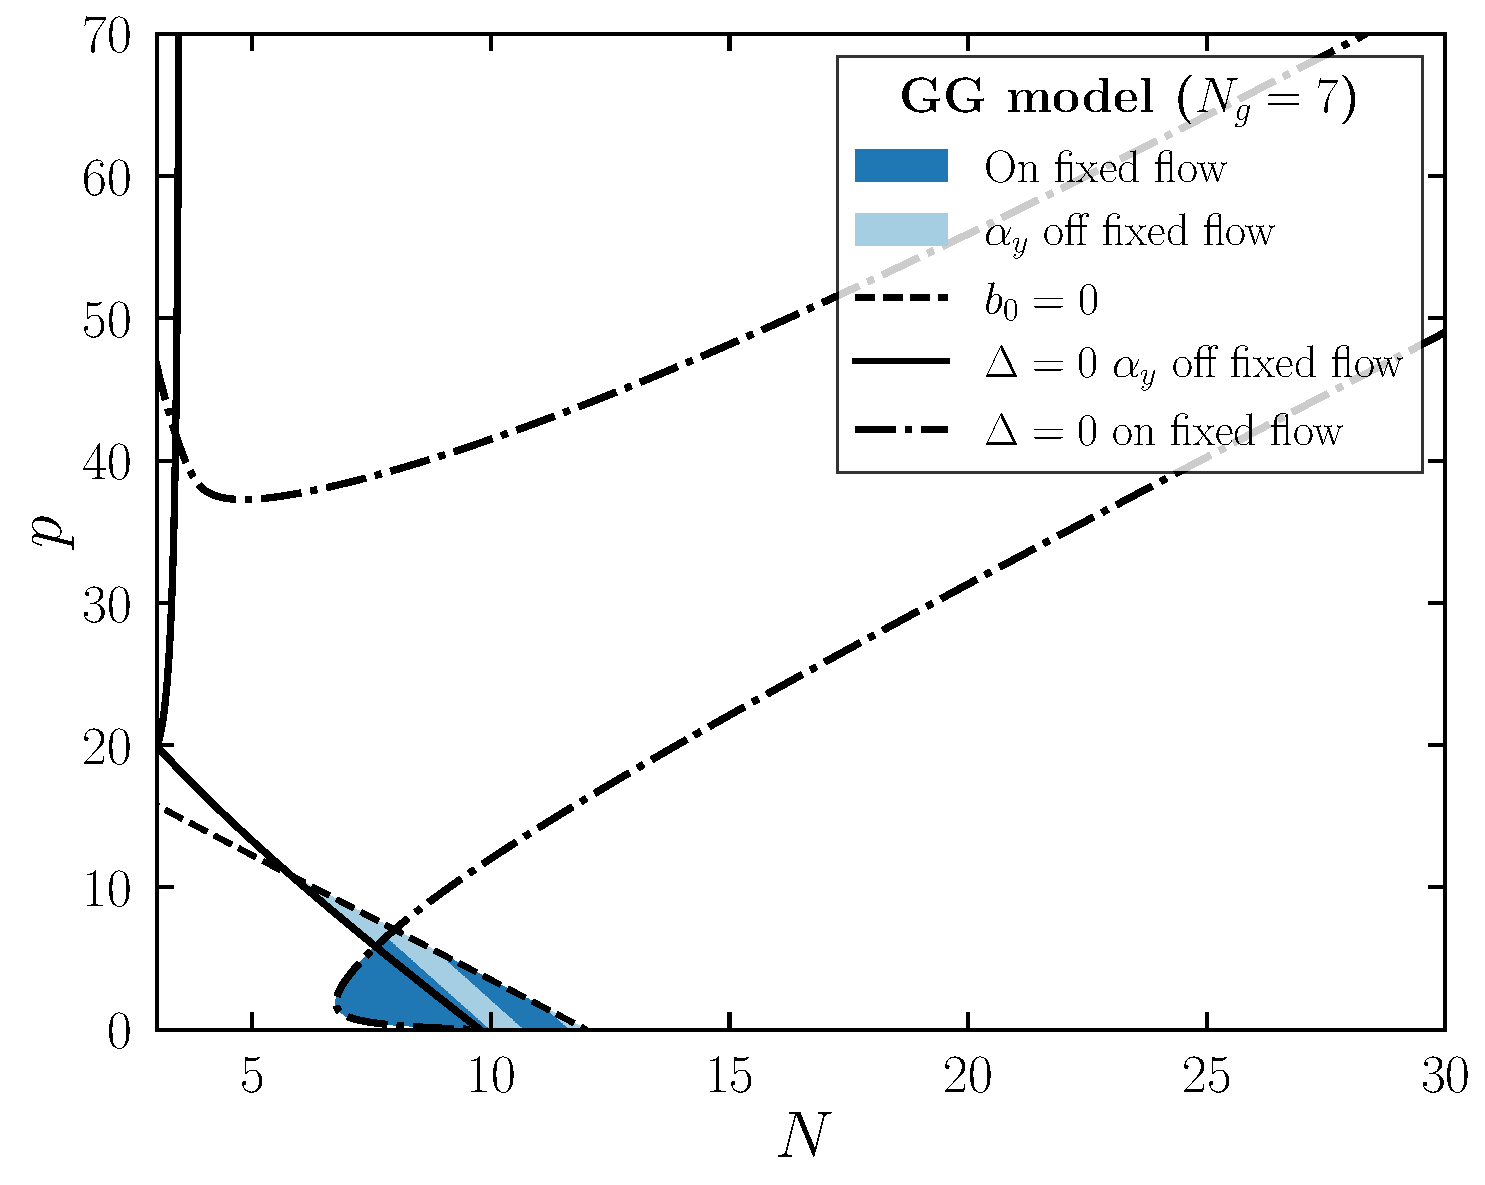
\includegraphics[width=\textwidth]{Figures/CAFplotGG_3_FinalCombined_Ng7.pdf}
        \caption{CAF region with $N_g=7$}
        \label{fig:gg_combined_ng6}
    \end{subfigure}
    
    \caption{Properties of the GG model with $N_g=5$ chiral families. (a) Root structure of the fourth-degree polynomial with all the couplings on fixed flow. The shaded regions denote four complex roots (white) or two real and two complex roots (light green). (b,c,d) CAF regions with all couplings on fixed flow (dark blue) and for the Yukawa coupling $\alpha_y$ off fixed flow (light blue). The dashed black line illustrates the $b_0=0$ condition (Eq.\ \eqref{eq:pmaxadj}), the solid black line the $\Delta=0$ for $\alpha_y$ off fixed flow \eqref{eq:Delta0noY} and the dash dotted line illustrates $\Delta=0$ on fixed flow \eqref{eq:Delta0}. } 
    \label{fig:Ng3}
\end{figure}

\begin{figure}[t!]
    \centering
    \begin{subfigure}[b]{0.49\textwidth}
        \centering
        
\includegraphics[width=\textwidth]{Figures/CAFplot_3_FinalCombined_Ng1.pdf}
        \caption{$N_g=1$} 
        \label{fig:gg_combined_ng1}
    \end{subfigure}
    \hspace{0.1cm}
    \begin{subfigure}[b]{0.49\textwidth}
        \centering
        
\includegraphics[width=\textwidth]{Figures/CAFplot_3_FinalCombined_Ng2.pdf}
        \caption{$N_g=2$} 
        \label{fig:gg_combined_ng3}
    \end{subfigure}
    
    \vspace{0.5cm} 
    \begin{subfigure}[b]{0.49\textwidth}
        \centering
        
\includegraphics[width=\textwidth]{Figures/CAFplot_3_FinalCombined_Ng3.pdf}
        \caption{$N_g=3$} 
        \label{fig:by_combined_ng5}
    \end{subfigure}
    \hspace{0.1cm}
    \begin{subfigure}[b]{0.49\textwidth}
        \centering
        
\includegraphics[width=\textwidth]{Figures/CAFplot_3_FinalCombined_Ng4.pdf}
        \caption{$N_g=4$}
        \label{fig:by_combined_ng6}
    \end{subfigure}
    
    \caption{CAF regions in the ($N$, $p$) parameter space for the BY model with $N_g \in \{1, 2, 3, 4\}$. The dark blue area indicates the region of CAF on the fixed flow, which is bounded above by the $b_0=0$ condition (dashed black line) \eqref{eq:padjscalar} and below by $\Delta=0$ (black dash dotted line) with $\alpha_y$ on fixed flow \eqref{eq:Delta0}. The light blue area highlights the region of CAF with the Yukawa coupling $\alpha_y$ off the fixed flow, bounded by the $b_0=0$ above and $\Delta=0$ below (solid black line) for $\alpha_y$ off fixed flow \eqref{eq:Delta0noY}. } 
    \label{fig:GGadjNG37}
\end{figure}
Matters change when the number of families is $N_g=5$. In Figure \ref{fig:roots_fixed_ng3}, the nature of the roots is shown, which has a region of two real and two complex roots within the region of an asymptotically free gauge coupling. Further, the polynomial has one sign change in this area, and thus has one positive real root as a consequence of Descartes' rule of signs. As seen in Figure \ref{fig:final_combined_ng3}, there is a CAF region on fixed flow.

Off fixed flow, we have a similar region to the case of $N_g=(1,2)$ and the combined CAF regions are shown in Figure \ref{fig:final_combined_ng3}, where the light blue region is the region off fixed flow and the dark blue region is on fixed flow. A similar case is that of $N_g=6,7$, which can be seen in Figure \ref{fig:gg_combined_ng5} and \ref{fig:gg_combined_ng6}. For $N_g>13$, the gauge coupling loses asymptotic freedom.

As we saw in Section \ref{sec:fundscalarNg}, the BY model exhibited CAF for $N_g<5$. The same is the case when adding an adjoint scalar. In Figure \ref{fig:GGadjNG37}, the CAF region can be seen for the case of $N_g\in\{1,2,3,4\}$.

Having examined the consequences of the Yukawa coupling off fixed flow, we now turn to a complementary scenario in the scalar sector. Specifically, we consider one quartic coupling off fixed flow and analyse whether this model exhibits CAF trajectories. Furthermore, we consider the case of both one quartic and one Yukawa coupling off fixed flow. 

% \subsection{One Quartic Scalar Coupling off Fixed Flow}
% Let us turn our focus to the scalar sector and consider one quartic coupling off fixed flow. We first take $\alpha_{\lambda_1}$ off fixed flow, effectively decoupling the quartic beta functions, we obtain
% \begin{align}
%     \beta_{{\lambda_1}} &=3N\alpha_g^2-2p\alpha_{y}^2\;,
%     \\
%     \beta_{{\lambda_2}}&=(7+N^2)\alpha_{\lambda_2}^2+4(p\alpha_{y}-3N\alpha_{g})\alpha_{\lambda_2}+18\alpha_{g}^2\;.
% \end{align}
% We can use the CAF conditions from Section \ref{sec:CAGquartic}, in Eqs. \eqref{eq:CAFfixednolam1} and \eqref{eq:CAFnotfixednolam1}. The new condition introduced in this CAF analysis for $\alpha_{\lambda_1}$ is $d_4''<0$ or $d_4<0$, depending on whether the Yukawa coupling is on or off fixed flow, respectively. In this case, $d_4=3N$, which will never be negative. Thus, a model with one adjoint scalar, which has both $\alpha_{\lambda_1}$ and $\alpha_y$ off fixed flow, cannot be CAF.
% In the case of only $\alpha_{\lambda_1}$ off fixed flow, the new condition in this model will be
% \begin{align}
%     d_4''=3N-2K\left(\frac{b_0-c_1}{c_2}\right)^2<0\;.
% \end{align}
% This condition will only be satisfied in regions where the CAF condition $k_e'<0$ holds. Thus, the theory cannot be CAF in the case of only $\alpha_{\lambda_1}$ off fixed flow. 

% In the case of $\alpha_{\lambda_2}$ off fixed flow, the condition is $e_4''<0$ and $e_4<0$. For this theory, we have the constraints
% \begin{align}
%     18&=e_4<0\;,\\
%     18&+\frac{12(3+N^2)}{N^2}\left(\frac{b_0-e_2\pm\sqrt{k_e}}{2e_1}\right)^2=e''_4<0\;.
% \end{align}
% Neither of these conditions will be satisfied for any $(N,p)$. 

% In conclusion, only with all the couplings or the Yukawa coupling $\alpha_{y}$ off fixed flow can the theory exhibit CAF. 

